%%%%%%%%%%%%%%%%%%%%%%%%%%%%%

% Modificación de la plantilla original de esta url: 
% https://www.overleaf.com/latex/templates/tesis-ipn-cic/xqrvnwbtqfnw

% Adaptada para la ESIME IPN.
% Cualquier sugerencia, corrección o comentario a: https://github.com/rulzco

% La plantilla requiere de :
% \usepackage{titlePage} y el archivo titlepage.sty en el mismo directorio de trabajo.
% y los campos (sin signo %) :

\documentclass[letterpaper,12pt,oneside]{book}
%\usepackage[top=1in, left=1.25in, right=1.25in, bottom=1in]{geometry} % Tamaño de papel y margen
\usepackage{lipsum}
\usepackage[top=1in, left=0.9in, right=1.25in, bottom=1in]{geometry}
\usepackage{titlePage}
\usepackage{subfiles}
%\usepackage{titlesec} % remueve la palabra «Capítulo» de \chapter
%\titleformat{\chapter} % Config titlesec
%	{\Large\bfseries}	% 
%	{\huge \thechapter}	% 
%	{20pt}				% 
%	{\huge}				% 
\usepackage[titletoc]{appendix} % Añade palabra «Apéndice» en Índice y define el ambiente appendices
\setlength{\parindent}{0em} % espacio de la sangría
\setlength{\parskip}{1em} % espacio entre párrafos
\usepackage[margin=10pt,font=small,labelfont=bf]{caption}
%\captionsetup{font=small} % Tamaño fuente 10pt en caption
\usepackage[utf8]{inputenc}
\usepackage[spanish,es-nodecimaldot,es-tabla]{babel}
%\usepackage{lmodern}
\usepackage[T1]{fontenc}
\usepackage{fancyhdr}
\usepackage{url}
\usepackage{ifthen}
\usepackage{multicol} % páginas con múltiples columnas
\usepackage{multirow} % tablas con múltiples filas
\usepackage{doi}
\usepackage{url}
\usepackage{booktabs}  % tablas de mayor calidad
\usepackage{graphicx} 
\usepackage{tikz} % crear elementos gráficos en LaTeX
\usepackage{tocloft} % tipografía de Tabla de contenidos, lista de figuras,lista de tablas
\usepackage{caption}
\usepackage{subcaption}
\graphicspath{{figs/}}
\usepackage{setspace}
\usepackage{comment} % comentarios de bloques
\usepackage{hyperref}
\urlstyle{same}
\hypersetup{
   bookmarksopen = true,
   bookmarksnumbered = true,
   breaklinks = true,
   colorlinks=true,
   urlcolor=cyan,
   linkcolor=black,
   citecolor=red,
   filecolor=magenta,
   pdftitle={Sharelatex Example},
   pdfpagemode=FullScreen,
}

%\usepackage[natbibapa]{apacite} % citar estilo APA
\usepackage[square, sort, numbers,colon ]{natbib}  

\usepackage{xcolor} % definir colores
\definecolor{Verde}{RGB}{0,133,60}
\definecolor{Plata}{RGB}{155,162,168}

\usepackage{amsmath,amsfonts} % ecuaciones y símbolos matemáticos
\usepackage[spanish]{cleveref}% \cref >> considera el tipo de ambiente usado.
\crefname{table}{Tabla}{Tablas}
%\crefname{equation}{Ec.}{Ec.}
%\crefname{figure}{Fig.}{Fig.}
\usepackage{longtable} % tablas extensas
\usepackage{breqn} % dividir ecuaciones largas con dmath
\usepackage{dirtree} % arboles de directorios
\usepackage{listingsutf8}  % insertar código
\definecolor{codegreen}{rgb}{0,0.6,0}
\definecolor{codegray}{rgb}{0.5,0.5,0.5}
\definecolor{codepurple}{rgb}{0.58,0,0.82}
\definecolor{backcolour}{rgb}{0.95,0.95,0.92}
\lstdefinestyle{myStyle}{ %definir el estilo del código
    language=C++,
    backgroundcolor=\color{backcolour},   
    commentstyle=\color{codegreen},
    keywordstyle=\color{magenta},
    numberstyle=\tiny\color{codegray},
    stringstyle=\color{codepurple},
    basicstyle=\ttfamily\footnotesize,
    breakatwhitespace=false,         
    breaklines=true,                 
    keepspaces=true,                 
    numbers=left,       
    numbersep=5pt,                  
    showspaces=false,                
    showstringspaces=false,
    showtabs=false,                  
    tabsize=2,
}

\usepackage{physics,siunitx} % physics define cosas como \pdv para derivadas parciales, notación de Dirac y demás. siunitx tiene una descripción para "desesperados" en su documentación que es bastante útil.
\sisetup{ % Config. global de Siunitx
open-bracket = {},close-bracket = {}, % quita paréntesis de números 
range-phrase = {\translate{ a }}, % Traduce "to" a español
list-final-separator = {\translate{ y }}, % Traduce "and" a español
list-pair-separator = {\translate{ y }}, % Traduce "and" a español
%parse-numbers = false, % Poder usar formato S con datatool en tablas
table-number-alignment = center-decimal-marker, % Alinea al centro el punto decimal en tablas
per-mode = symbol
}

% encabezados personalizados
%\pagestyle{fancy}
%\addtolength{\headheight}{12.5pt}
%\renewcommand{\chaptermark}[1]{\markboth{\MakeUppercase{\thechapter. #1 }}{}}
%\renewcommand{\sectionmark}[1]{\markright{\thesection\ #1}}
%\fancyhf{}
%\fancyhead[RO]{\rightmark}
%\fancyhead[LE]{\leftmark}
%\fancyfoot[C]{\thepage}
%\renewcommand{\headrulewidth}{0.5pt}
%\renewcommand{\footrulewidth}{0.1pt}

%\addtolength{\headheight}{12.5pt}
%\fancypagestyle{plain}{
%  \fancyhead{}
%  \renewcommand{\headrulewidth}{0pt}
%}

%\renewcommand\cftsecpresnum{\S}
%\renewcommand\cftsubsecpresnum{\S}

%%%%%%%%%%%%%%%%%%%%%%%%%%%%%
% Definir los campos de la portada
% y los campos (sin signo %) :
\author{M.en C.}
\title{Título de la tesis} 
\faculty{Escuela Superior de Ingeniería Mecánica y Eléctrica, \\Unidad Zacatenco} % escuela
\degree{Dr. en Ciencias} % grado a obtener
\supervisor{ Tutor} % directores
\cityandyear{Ciudad de México \\20--} % lugar y fecha
\logouni{escudoIPN} %logo IPN
\logofac{escudoESIME} % logo ESIME
%%%%%%%%%%%%%%%%%%%%%%%%%%%%%

\begin{document}

\frontmatter
\maketitle % crea la carátula
%\begin{titlepage}
  \thispagestyle{empty}
  \begin{minipage}[c][0.17\textheight][c]{0.25\textwidth}
    \begin{center}
      
\includegraphics[ height=4cm]{figs/escudoIPN.pdf}
    \end{center}
  \end{minipage}
  \begin{minipage}[c][0.195\textheight][t]{0.75\textwidth}
    \begin{center}
      \vspace{0.3cm}
             {\color{black}\textsc{\large Instituto Politécnico Nacional} }\\[0.5cm]
             \vspace{0.3cm}
                    {\color{Verde}\hrule height2.5pt}
                    \vspace{.1cm}
                           {\color{Plata}\hrule height1.pt}
                           \vspace{.8cm}
                           \textsc{Escuela Superior de Ingeniería Mecánica y Eléctrica, \\ Unidad Zacatenco }\\[1cm] %
    \end{center}
  \end{minipage}
  \begin{minipage}[c][0.81\textheight][t]{0.25\textwidth}
    \vspace*{5mm}
    \begin{center}
      \hskip2.0mm
             {\color{Verde}\vrule width 2.5pt height 13cm}
             \hskip -0.4mm
                 {\color{Plata}\vrule width 1pt height 13cm} \\
                 \vspace{5mm}
                 
\includegraphics[height=3.0cm]{figs/escudoESIME.pdf}
    \end{center}
  \end{minipage}
  \begin{minipage}[c][0.81\textheight][t]{0.75\textwidth}
    \begin{center}
      \vspace{1cm}

      {\color{red}{\large\scshape Titulo de la Tesis }}\\[.2in]

      \vspace{2cm}            

      %\textsc{\Huge T\hspace{0.5cm}E\hspace{0.5cm}S\hspace{0.5cm}I\hspace{0.5cm}S}\\[2cm]
      
      \makebox[8cm][s]{\Large\bfseries T E S I S}\\[1.2cm]
      \makebox[7cm][c]{QUE PARA OBTENER EL GRADO DE:}\\[0.8cm]
      %\textsc{\large QUE PARA OBTENER EL GRADO DE:}\\[0.5cm]
      \textsc{\large Dr. en Ciencias en Ingeniería Mecánica}\\[0.7cm]
      
      {\color{black}\textsc{\large presenta:}}\\[0.5cm]
      \textsc{\large {M. en C.}}\\[1cm]          

      \vspace{0.5cm}
      
	  %QUE PARA OBTENER EL GRADO DE:\\[5pt]
      %\textbf{Dr. en Ciencias en Ingeniería Mecánica}\\[40pt]
	  %PRESENTA:\\[5pt]
	  %\textbf{M. en C.}

      {\normalsize\scshape 
        {\color{black}Directores:}\\[0.3cm] {Dr.  \\ 
          Dr. }}\\[.2in]

      \vspace{1cm}

      \large{Ciudad de México\\
        2021}
    \end{center}
  \end{minipage}
\end{titlepage}
%--------------------------------- %  carátula alternativa
%------------------------------------------
% DEDICATORIA
%------------------------------------------
\chapter*{}
%\vspace{2cm}
\begin{flushright}
	{\fontfamily{ppl}%Palatino
	\selectfont\emph{<<It's the questions we can't answer that teach us the most. They teach us how to think. If you give a man an answer, all he gains is a little fact. But give him a question and he'll look for his own answers.>>}\\
\vspace{5mm}
	Patrick Rothfuss}

\end{flushright}
\vfill
%------------------------------------------
% AGRADECIMIENTOS
%------------------------------------------
\chapter{Agradecimientos}
\lipsum[6-9]


% enlaces de color negro en la tabla de contenidos y lista de figuras
%{
%  \hypersetup{linkcolor=black}
%  \tableofcontents
%  \listoffigures
%}
\tableofcontents
\listoffigures

\chapter{Notación}


\chapter{Introducción}

\lipsum[1-9]

%------------------------------------------
% CAPÍTULOS
%------------------------------------------
\mainmatter
\chapter{Marco teórico}

\section{Ecuaciones y citarlas}

\begin{comment}
  Objetivo: Explicarles a los lectores de computación que entienden
  los lingüistas de una variación dialectal
\end{comment}

Divergencia de $\vec{u}$ \eqref{eq:divergence}, ecuación de Navier-Stokes \eqref{eq:NavierStokes}. La \cref{tab:dielectricK}

Citar usando cref:

En las \cref{fig:Cpx_rans_8,fig:Cpx_rans_10} , las \cref{eq:divergence,eq:NavierStokes} En la  \cref{tab:dielectricK}... En el \cref{c:codigo}

\begin{equation}\label{eq:divergence}
    \nabla\cdot \vec{u}
\end{equation}

\begin{equation}\label{eq:NavierStokes}
\frac{\partial \bar{u_i}}{\partial t} +\bar{u_j}\frac{\partial \bar{u_i}}{\partial x_j}=-\frac{1}{\rho}\frac{\partial \bar{p}}{\partial x_i}+\nu\frac{\partial^2 \bar{u_i}}{\partial x_j^2}+\frac{f_b}{\rho}
\end{equation}

Dividir una ecuación larga usando dmath del paquete breqn:

\begin{dmath}\label{eq:reynolds:_transport}
\frac{\partial}{\partial t}\left \langle u_i u_k\right \rangle+U_j\frac{\partial}{\partial x_j}\left \langle u_i u_j\right \rangle = \frac{p}{\rho}\left[\frac{\partial u_i}{\partial x_k}+\frac{\partial u_k}{\partial x_i} \right]+\frac{\partial}{\partial x_j}\left \{ -\frac{1}{\rho}\left[ \left \langle pu_k\right \rangle\delta_{ij}+\left \langle pu_i\right \rangle\delta_{kj}\right] -\left \langle u_i u_j u_k\right \rangle+ 2\nu\left [ s_{ij}u_k+s_{ikj}u_i \right ] \right \}-\left [ u_i u_j \frac{\partial U_k}{\partial x_j}+u_k u_j \frac{\partial U_i}{\partial x_j} \right ]-2\nu\left [ s_{ij} \frac{\partial u_k}{\partial x_j}+s_{kj}\frac{\partial u_i}{\partial x_j} \right ]
\end{dmath}

\subsection{Unidades con el paquete siunitx}

La gravedad tiene una aceleración de \SI{9.8}{ms^{-2}},\\
\si{\kilo\gram\metre\per\square\second} \\
\si{\gram\per\cubic\centi\metre}\\        \si{\square\volt\cubic\lumen\per\farad}\\
\si{\metre\squared\per\gray\cubic\lux} \\ 
\si{Hs}\\
\SI{200}{GHz}

Para mas detalles consultar \href{https://ctan.mirrors.hoobly.com/macros/latex/contrib/siunitx/siunitx.pdf}{Manual de usuario de siunitx}.

\subsection{Citar una referencias}

Diferentes formas de citar a una referencia o autor \citet{abdollahzadeh2016implementation}, Suzen \cite{suzen_numerical_2005} y citar el año de publicación del trabajo \citeyear{dorr_numerical_2015}:

\section{Tablas}



Ejemplo de una Tabla \ref{tab:dielectricK}.

\begin{table}[!ht]
\centering
\caption{Permitividad relativa de diferentes dieléctricos}
\label{tab:dielectricK}
\begin{tabular}{@{}cc@{}}
\toprule
Material           & Permitividad Relativa ($\varepsilon_r$)\\ \midrule
Aire               & 1.0                   \\
Kapton (Poliimida) & 3.4                   \\
Plexiglas          & 4.7                   \\
Teflón             & 2.7                   \\
Vidrio             & 6.7                   \\ \bottomrule
\end{tabular}
\end{table}

\section{Figuras}

Una figura simple \ref{fig:Cpx_rans_14}. Las subfiguras, se pueden citar individualmente  y \ref{fig:Cpx_rans_10} o en su conjunto \ref{fig:Cpx_rans_a2}.

\begin{figure}[ht!]
  \centering
    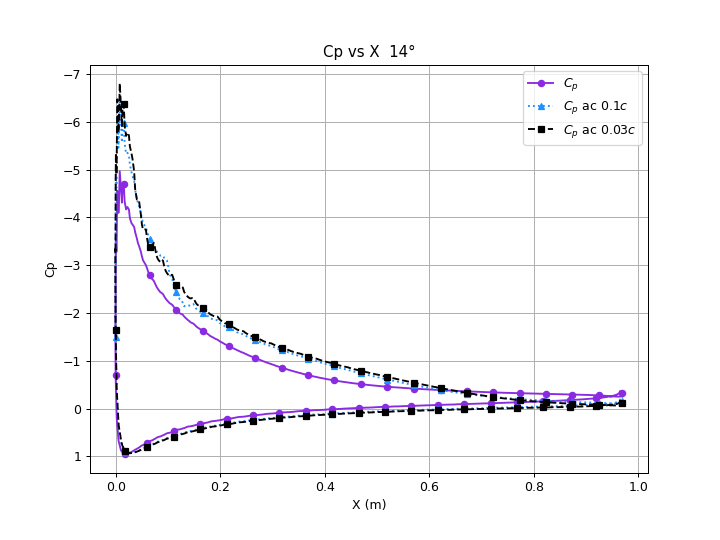
\includegraphics[width=0.75\textwidth]{Cpx_rans_14}    
    \caption{Distribución de coeficientes de presión.}         
  \label{fig:Cpx_rans_14}                          
\end{figure}


\begin{figure}[ht!]
\centering
\begin{subfigure}{0.5\textwidth}
  \centering
  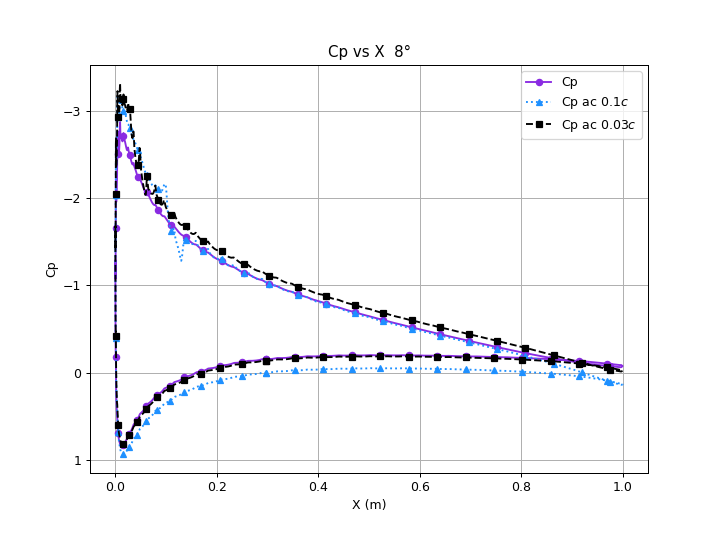
\includegraphics[width=1.0\textwidth]{Cpx_rans_8}
  \caption{Distribución de Cp para $\alpha=8^\circ$.}
  \label{fig:Cpx_rans_8}
\end{subfigure}%
\begin{subfigure}{0.5\textwidth}
  \centering
  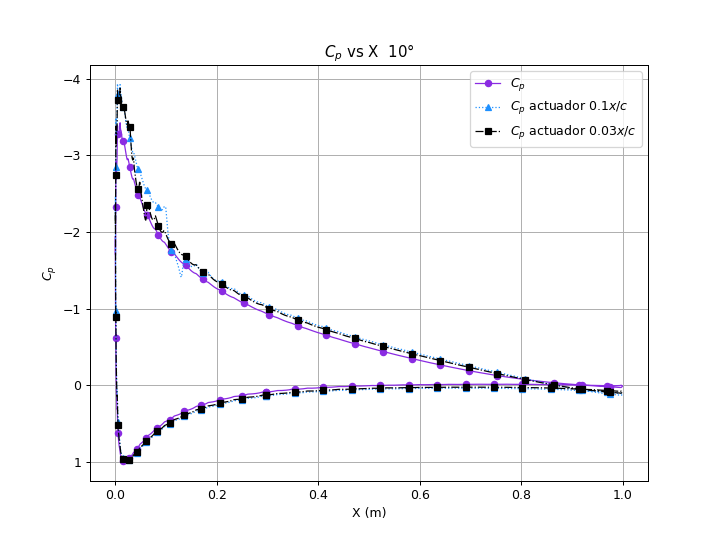
\includegraphics[width=1.0\textwidth]{Cpx_rans_10}
  \caption{Distribución de Cp para $\alpha=10^\circ$.}
  \label{fig:Cpx_rans_10}
\end{subfigure}
\caption{Distribución de presión sobre la superficie del perfil.}
\label{fig:Cpx_rans_a2}
\end{figure}    

\subsection{Arboles de directorios}

Es posible crear arboles de directorios:

\dirtree{%
.1 icoFoam.
.2 Make.
.3 files.
.3 options.
.2 createFields.H.
.2 icoFoam.C.
}

\chapter{Estado del arte}
\chapter{Avances}

\section{Redes sociales, especialmente Twitter como fuente de datos geolingísticos}
\subsection{Metadatos generales de Twitter}
\subsubsection{Metadatos geográficos de Twitter}

\section{Descripción de los datos recogidos}
{\color{red} Los nombres propuestos para los corpus no son los oficiales,
  es importante consultar como llamar y sobretodo como citar el segundo
corpus}
\subsection{Corpus de Tweets panispánicos}
\subsection{Corpus de Tweets geolocalizados de Claremont-Riverside}

\chapter{Problema de Investigación}
Durante la maestría se trabajó el cambio lingüístico a nivel léxico
sin profundizar en otros niveles de la lengua que tambien se pueden
explorar con datos de texto (Niveles  morfo-fonológico, morfo-sintáctico,).
Se inició una exploración inicial del nivel semántico mediante la
creación de WordEmbeddings y se realizaron pequeños experimentos
de analogías geográficas usando topónimos como miembos de la analogía,
pero no se exploraron las posibilidades de la información geográfica.


\textbf{Nota}: {\color{red}Revisar esta sugerencia de Segun:} \href{https://github.com/INGEOTEC/RegionalEmbeddings}{FastText Word Embeddings for Spanish Language Variations} 


[Objetivo: ]



\backmatter%@sglvgdor
\chapter{Conclusiones}
\lipsum[6-9]

%------------------------------------------
% APÉNDICES
%------------------------------------------
\begin{appendices}
\appendix
%\documentclass[../Main.tex]{subfiles}
\begin{document}
%\chapter{Insertar código}\label{apen:1}
\label{c:codigo}

\begin{lstlisting}[style=myStyle,firstnumber=58]
        // Momentum predictor

        fvVectorMatrix UEqn
        (
            fvm::ddt(U)
          + fvm::div(phi, U)
          - fvm::laplacian(nu, U)
        );
\end{lstlisting}

Código desde un archivo: 

\lstinputlisting[language=C++,numbers=left,,frame=L, firstline=1, lastline=20]{createFields.H}

\end{document}
\chapter{Insertar código}
\subfile{apendices/ap1}

\end{appendices}


%\bibliographystyle{apacite}
\bibliographystyle{unsrtnat}
\bibliography{References/refs.bib}


\end{document}
